%% USEFUL LINKS:
%% -------------
%%
%% - UiO LaTeX guides:          https://www.mn.uio.no/ifi/tjenester/it/hjelp/latex/
%% - Mathematics:               https://en.wikibooks.org/wiki/LaTeX/Mathematics
%% - Physics:                   https://ctan.uib.no/macros/latex/contrib/physics/physics.pdf
%% - Basics of Tikz:            https://en.wikibooks.org/wiki/LaTeX/PGF/Tikz
%% - All the colors!            https://en.wikibooks.org/wiki/LaTeX/Colors
%% - How to make tables:        https://en.wikibooks.org/wiki/LaTeX/Tables
%% - Code listing styles:       https://en.wikibooks.org/wiki/LaTeX/Source_Code_Listings
%% - \includegraphics           https://en.wikibooks.org/wiki/LaTeX/Importing_Graphics
%% - Learn more about figures:  https://en.wikibooks.org/wiki/LaTeX/Floats,_Figures_and_Captions
%% - Automagic bibliography:    https://en.wikibooks.org/wiki/LaTeX/Bibliography_Management  (this one is kinda difficult the first time)
%%
%%                              (This document is of class "revtex4-1", the REVTeX Guide explains how the class works)
%%   REVTeX Guide:              http://www.physics.csbsju.edu/370/papers/Journal_Style_Manuals/auguide4-1.pdf
%%
%% COMPILING THE .pdf FILE IN THE LINUX IN THE TERMINAL
%% ----------------------------------------------------
%%
%% [terminal]$ pdflatex report_example.tex
%%
%% Run the command twice, always.
%%
%% When using references, footnotes, etc. you should run the following chain of commands:
%%
%% [terminal]$ pdflatex report_example.tex
%% [terminal]$ bibtex report_example
%% [terminal]$ pdflatex report_example.tex
%% [terminal]$ pdflatex report_example.tex
%%
%% This series of commands can of course be gathered into a single-line command:
%% [terminal]$ pdflatex report_example.tex && bibtex report_example.aux && pdflatex report_example.tex && pdflatex report_example.tex
%%
%% ----------------------------------------------------


\documentclass[english,notitlepage,reprint,nofootinbib]{revtex4-1}  % defines the basic parameters of the document
% For preview: skriv i terminal: latexmk -pdf -pvc filnavn
% If you want a single-column, remove "reprint"

% Allows special characters (including æøå)
\usepackage[utf8]{inputenc}
% \usepackage[english]{babel}

%% Note that you may need to download some of these packages manually, it depends on your setup.
%% I recommend downloading TeXMaker, because it includes a large library of the most common packages.

\usepackage{physics,amssymb}  % mathematical symbols (physics imports amsmath)
\include{amsmath}
\usepackage{graphicx}         % include graphics such as plots
\usepackage{xcolor}           % set colors
\usepackage{hyperref}         % automagic cross-referencing
\usepackage{listings}         % display code
\usepackage{subfigure}        % imports a lot of cool and useful figure commands
% \usepackage{float}
%\usepackage[section]{placeins}
\usepackage{algorithm}
\usepackage[noend]{algpseudocode}
\usepackage{subfigure}
\usepackage{tikz}
\usetikzlibrary{quantikz}
% defines the color of hyperref objects
% Blending two colors:  blue!80!black  =  80% blue and 20% black
\hypersetup{ % this is just my personal choice, feel free to change things
    colorlinks,
    linkcolor={red!50!black},
    citecolor={blue!50!black},
    urlcolor={blue!80!black}}


% ===========================================


\begin{document}

\title{How to write a scientific report}  % self-explanatory
\author{The names of the authors go here} % self-explanatory
\date{\today}                             % self-explanatory
\noaffiliation                            % ignore this, but keep it.

%This is how we create an abstract section.
\begin{abstract}
    We provide an overview of how to structure a scientific report. For concreteness, we consider the example of writing a report about an implementation of the midpoint rule of integration. For each section of the report we briefly discuss what the purpose of the given section is. We also provide examples of how to properly include equations, tables, algorithms, figures and references.
\end{abstract}
\maketitle


% ===========================================
\section{Introduction}
%
The purpose of this report template is two-fold: to communicate how to write a scientific report on a numerical topic, while simultaneously provide a concrete ``minimal working example'' of such a report. As our example topic we will look at an implementation of something rather dull and simple, namely the \textit{midpoint rule for integration}.

Throughout this example we will provide (hopefully) pedagogical commentary on report writing and structure, while at the same time present the midpoint rule for integration in a proper manner. To avoid confusion, we will from now on put pedagogical commentary in \textit{italics}. The next paragraph could have been part of the report, but we will leave it as a pedagogical comment: \textit{Writing reports, or papers, is a fundamental part of the scientific enterprise. It is vital to properly communicate precisely what has been done, what the results are and their implications. The motivation for this is to make the work understood and reproducible, so that others can both check and build on your work.}

\textit{The main purpose of the introduction section is to provide context and motivation for the work, like we have done above. It is also common --- and quite useful --- to use the last paragraph of the introduction to outline the rest of the report, to tell the reader what they should expect in the different sections. We will do this next.}

In section \ref{sec:methods} we describe the mathematical background and formulate a concrete algorithm which can be implemented in any programming language. A selection of results from a validation test are presented in section \label{sec:results}. In section \label{sec:discussion} we discuss our implementation of the algorithm in more detail, and in section \ref{sec:conclusion} we provide a short summary and outlook.

\textit{Now, since the toy example we study here is rather short and simple, our outline isn't particularly detailed. But for a report that is longer, a slightly more detailed outline might be useful.}


% ===========================================
\section{Methods}\label{sec:methods}
%
\textit{The main purpose of the ``Methods'' (or ``Theory'', or ``Algorithms'') section is to provide the reader with the necessary background knowledge to understand the work you will present.\footnote{Note that to get correct quotation marks in LaTeX, you cannot simply use the quotation mark symbol on your keyboard. Check the \texttt{.tex} file for this document to see the correct approach.} It should in general be sufficiently detailed for the reader to understand and reproduce what you have done. However, sometimes it can be a good idea to relegate the discussion of some technical topic to an appendix, to avoid too long discussions of what might be a a fairly minor or technical detail. You are of course free to divide this section into subsections, which we will do below.}

Let $f$ be a continuous and differentiable function, $f: [a,b] \to \mathbb{R}$. Say we want to integrate this function over the entire interval $[a,b]$. To this end, we employ the midpoint rule for integration, which is defined by the equation~\cite{midpoint_rule}
%
\begin{equation}
    I = \int_a^b f(x)\dd x \approx h\sum_{i=1}^{n} f(x_i).
\end{equation}
Here $n$ denotes a number of subintervals of the range $[a,b]$, each of length $h = (b-a)/n$, and $x_i$ is the midpoint of subinterval $i$, given by
\begin{equation}
   x_i = a + \left(i-\frac{1}{2}\right) h,
\end{equation}
for $i = 1, 2, \ldots, n$. This equation can be written out explicitly (although in this case it is a bit silly):
%
\begin{equation}
    \begin{split}
        \int_a^b f(x)\dd x & \approx h \sum_{i=1}^{n} f(x_i) \\
                                    \\
                                    & = h\left(f(x_1) + \cdots + f(x_{n})\right).
    \end{split}
\end{equation}
%
\textit{Note the following: We have provided a definition for every single variable that appears in the equations. Always do this --- it greatly improves the transparency and readability of your work! Once a variable is defined, you can reuse it throughout the rest of the report without stating its definition. (This of course assumes that you use consistent notation, so that a symbol does not suddenly change meaning in the middle of your report.)}

\textit{Also, note that we cited a source for our claim. There is no need to provide references for trivial or very well-known results, like Newton's second law, but you should cite material that is vital for your report.}

\textit{Finally, please note the following two details on how to write equations: First, remember that equations are regarded as part of a sentence, meaning that you should follow the standard rules for punctuation. This typically means that your equations should be followed by a comma or a period. Second, make sure that you do not unintentionally include blank lines before or after the equation in your \texttt{.tex} file. LaTeX interprets blank lines as the beginning of a new paragraph, and will therefore indent the text after the equation. If you prefer having a bit of ``air'' in your LaTeX document, use empty comment line.}

To test our integration algorithm we will use it to integrate the polynomial $f(x) = x^3$ over the interval $[a,b] = [0,1]$. This is a suitable test case, since the integral has a known analytical solution,
\begin{equation}
    \int_0^1 x^3 \dd x = \frac{1}{4}.
\end{equation}
In assessing the performance of our approach we will consider the relative error $\epsilon$, defined as
\begin{equation}
    \epsilon = \abs{ \frac{I - I_{\text{approx}}}{I} },
\end{equation}
where $I$ denotes the exact integral and $I_\text{approx}$ denotes the approximation obtained with our implementation of the midpoint rule algorithm.


% ===========================================
\subsection*{The algorithm}
%
The algorithm for the midpoint rule is summarized in algorithm~\ref{algo:midpointrule}. The basic idea behind the algorithm is to divide the integration range into to $n$ small subintervals of length $h$, and on each such subinterval approximate the function $f(x)$ by a constant function. The value for this constant function is taken to be the value of $f(x)$ evaluated at the midpoint of the given subinterval --- hence the name of the method.
%
\begin{figure}
% NOTE: We only need \begin{figure} ... \end{figure} here because of a compatability issue between the 'revtex4-1' document class and the 'algorithm' environment.
    \begin{algorithm}[H]
    \caption{Midpoint rule for integration}
    \label{algo:midpointrule}
        \begin{algorithmic}
            \Procedure{Midpoint rule}{$f, a, b, n$}
            \State $I \leftarrow 0$        \Comment{Initialize the integral variable}
            \State $h \leftarrow (b-a)/n$  \Comment{Compute the interval length}
            \For{$i = 1, 2, \ldots, n$}
            \State $x \leftarrow a + (i-1/2)h$  \Comment{Assign $x$ to the midpoint}  %This means x is assigned the value x + ih/2.
            \State $I \leftarrow I + f(x)$  \Comment{Add contribution to integral} %Assign I to I + f(x)
            \EndFor
            \State $I \leftarrow Ih$  \Comment{Finalize the computation}
            \EndProcedure
        \end{algorithmic}
    \end{algorithm}
\end{figure}

\textit{As demonstrated in algorithm~\ref{algo:midpointrule}, it is conventional to present algorithms in a way that is independent of any specific programming language. This ensures that it is the logic behind the algorithm that remains in focus, rather than the syntax of a particular programming language. In algorithm~\ref{algo:midpointrule} we have also demonstrated a common notation: The right-to-left arrow ($\leftarrow$) means that we assign the value of everything on the right to the variable on the left. This is nothing but how the ``='' symbol functions in most programming languages, but the arrow notation makes it clear that we are in fact assigning a value, rather than stating that two things are equal.}


% ===========================================
\section{Results}\label{sec:results}
%
To test the midpoint rule algorithm, we perform the integration of $f(x)$ using different choices for the number of subintervals. The results are listed in table \ref{tab:midpointruletab}.\footnote{A general style recommendation is to avoid having vertical lines in tables. There are of course exceptions, but in most cases vertical lines will make a table less readable.}
%
\begin{table}[h!]
    \centering
    \caption{Approximate values for the integral of $f(x) = x^3$ on the interval $[0,1]$, as obtained with the midpoint rule with different numbers of integration subintervals.}
    \begin{tabular}{c@{\hspace{1cm}} c}
        \hline
        Number of subintervals & Integral value \\
        \hline
        $10^1$  &  0.3086 \\
        $10^2$  &  0.2550 \\
        $10^3$  &  0.2505 \\
        $10^4$  &  0.2500 \\
        % $10$  &  0.3086 \\
        % $100$  &  0.2550 \\
        % $1 000$  &  0.2505 \\
        % $10 000$  &  0.2500 \\
        \hline
    \end{tabular}\label{tab:midpointruletab}
\end{table}

In figure \ref{fig:rel_err} we show the relative error as a function of the number of subintervals $n$.
\begin{figure}[h!]
    \centering %Centers the figure
    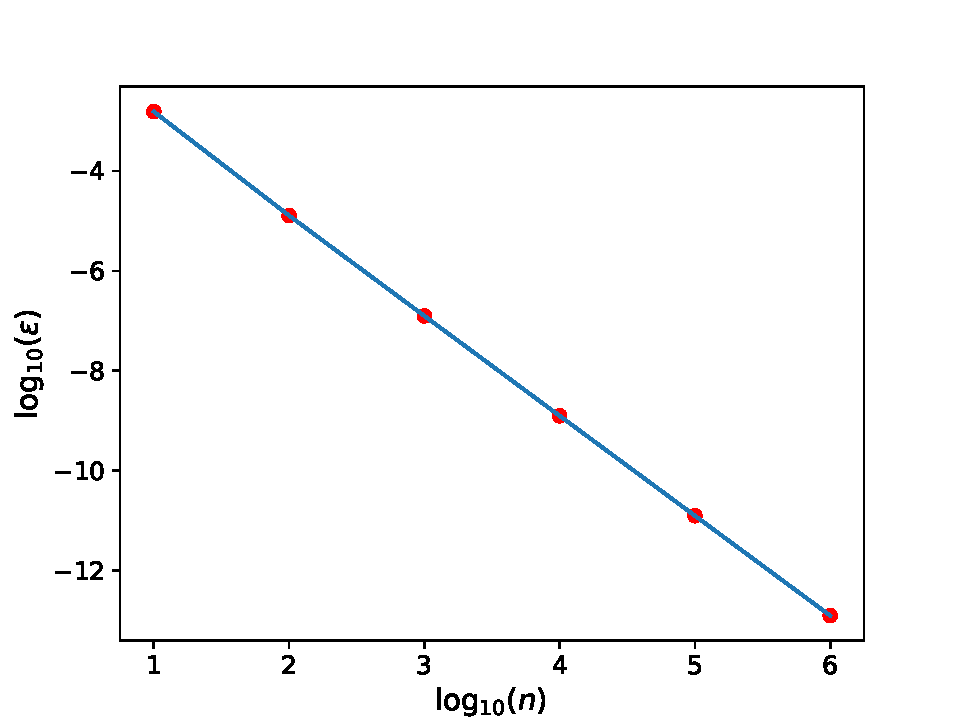
\includegraphics[scale=0.55]{imgs/rel_err.pdf} %Imports the figure.
    \caption{The relative error versus the number of integration subintervals ($n$) when using the midpoint rule to estimate the integral $\int_0^1 x^3\dd x$. \textit{Given that this plot is based only on a handful of data points, it should also show the data points using some form of point markers, like the dots here. When presented only with a continuous line, it is not necessarily clear for the reader if the result is based on a large or small number of data points.}}
    \label{fig:rel_err}
\end{figure}

\textit{Note especially how we reference both the table and the figure with a short explanation of their content. Always do this! In the figure/table captions we can also add additional information, such as information about how the figure/table was produced. You can also do this in the main text if you like. When writing the figure/table captions, keep in mind the general rule of thumb that an expert on the topic should be able to understand the gist of your report simply by reading the abstract and look at the figures/tables and read their corresponding captions.}


% ===========================================
\section{Discussion}\label{sec:discussion}
%
\textit{Note that you are free to merge the presentation and discussion of the results into a single section of your report. This can in many cases lead to a more fluid presentation. If you do this, we recommend you use ``Results and discussion'' or similar for the section title.}

From table \ref{tab:midpointruletab}, we note that our implementation reproduces the analytical results to four digits precision when the integration range is divided into $n = 10^4$ subintervals. This indicates that that our implementation of the algorithm is correct.

From figure \ref{fig:rel_err}, we see that $\log_{10}(\epsilon)$ decreases linearly with $\log_{2}(n)$. From this, it should be possible to extract the convergence rate of our implementation of the midpoint rule. From a theoretical point of view we know that the midpoint rule should have a convergence rate of $\mathcal{O}(h^2)$. To properly verify our implementation, we should have estimated the convergence rate from our results and compared it to this theoretical rate. Without doing so, we cannot know that the our implementation of the algorithm is correct, even though we have seen that the numerical approximation converges to the correct answer in \ref{tab:midpointruletab}.

\textit{Although this is a somewhat silly example, please note the following: We are to-the-point in our discussion of the results, and we only make strong claims about what we are actually certain about. In the discussion it is important to try to be as concise as possible --- long paragraphs that only make very general points are typically of limited interest. Note that we also highlight aspects of our analysis that could have been improved and that might form a topic for future work.}


% ===========================================
\section{Conclusion}\label{sec:conclusion}
\textit{In this section we state three things in a concise manner: what we have done, what we have found, and what should or could be done in the future.}

We have investigated an implementation of the midpoint rule for numerical integration. As a first validation test we have checked that our implementation of the method reproduces the analytical result for the definite integral of $f(x) = x^3$ on $x \in [0,1]$, achieving a four-digit precision when the integration range is divided into $n=10^4$ subintervals. Furthermore, we have presented results for how the relative error of the method varies with the number of subintervals. To use these results to extract a precise estimate for the convergence rate of the method remains a topic for future work. As such, while our implementation of the midpoint rule has passed the initial validation tests, more work is needed to fully assess the validity of the implementation.

\onecolumngrid

%\bibliographystyle{apalike}
\bibliography{ref}


\end{document}
